%%%%%%%%%%%%%%%%%%%%%%%%%%%%%%%%%%%%% 
%% LE2I beamer template
%% Guillaume Lemaitre, October 2014
%%%%%%%%%%%%%%%%%%%%%%%%%%%%%%%%%%%%% 

\documentclass{beamer}

\usepackage[utf8]{inputenc}
\usepackage[T1]{fontenc} 
\usetheme{le2i} 

%% The amssymb package provides various useful mathematical symbols
\usepackage{amssymb}
%% The amsthm package provides extended theorem environments
\usepackage{amsthm}
%% amsmath for math environment
\usepackage{amsmath}

\DeclareMathOperator*{\argmin}{arg\,min}
\DeclareMathOperator*{\argmax}{arg\,max}
\DeclareMathOperator*{\sign}{sign}

%% figure package
\usepackage{epsf,graphicx}
\usepackage{epstopdf}
\usepackage{subfigure}
\usepackage{transparent}

%% In order to draw some graphs
\usepackage{tikz,xifthen}
\usepackage{tikz-qtree}
\usepackage{adjustbox}
\usetikzlibrary{decorations.pathmorphing}
\usetikzlibrary{fit}
\usetikzlibrary{backgrounds}
\usetikzlibrary{shapes,arrows,shadows}
\usetikzlibrary{calc,decorations.pathreplacing,decorations.markings,positioning}
\usetikzlibrary{snakes,decorations.text,shapes,patterns}
% \usepackage{scalefnt,lmodern,booktabs}

%% Package for cross and tick symbols
\usepackage{pifont}
\newcommand{\tick}{\color{green!60!black!80}\ding{51}}
\newcommand{\cross}{\color{red!60!black!80}\ding{55}}

\setbeamercovered{transparent}
\resetcounteronoverlays{subfigure}
%remove the icon
\setbeamertemplate{bibliography item}{}

%remove line breaks
\setbeamertemplate{bibliography entry title}{}
\setbeamertemplate{bibliography entry location}{}
\setbeamertemplate{bibliography entry note}{}

\usepackage{multirow}
%\usepackage{biblatex}
%\addbibresource{bibtex.bib}

\title{\Large{A Boosting Approach for Prostate Cancer Detection using Multi-Parametric MRI}}
\author{\scriptsize{Guillaume Lemaitre \\ \texttt{guillaume.lemaitre@u-bourgogne.fr}}}
\date{\scriptsize{Quality Control by Artificial Vision \\ 4\textsuperscript{th} June 2015}}

\institute{Universit\'e de Bourgogne} 

\newenvironment<>{redblock}[1]{%
  \begin{actionenv}#2%
    \def\insertblocktitle{#1}%
    \par%
    \mode<presentation>{%
      \setbeamercolor{block title}{fg=nicewhite,bg=red!75!black}
      \setbeamercolor{block body}{fg=niceblack,bg=red!20}
    }%
    \usebeamertemplate{block begin}}
  {\par\usebeamertemplate{block end}\end{actionenv}}

\newenvironment<>{greenblock}[1]{%
  \begin{actionenv}#2%
    \def\insertblocktitle{#1}%
    \par%
    \mode<presentation>{%
      \setbeamercolor{block title}{fg=nicewhite,bg=green!40!black}
      \setbeamercolor{block body}{fg=niceblack,bg=green!20}
    }%
    \usebeamertemplate{block begin}}
  {\par\usebeamertemplate{block end}\end{actionenv}}

%% Uncomment if you want to avoid thousand of bullet inside the menu
% \usepackage{etoolbox}
% \makeatletter
% \patchcmd{\slideentry}{\advance\beamer@xpos by1\relax}{}{}{}
% \def\beamer@subsectionentry#1#2#3#4#5{\advance\beamer@xpos by1\relax}%
% \makeatother

\begin{document}

% Show the title page
\begin{frame}
  \titlepage
\end{frame}

% Show the table of contents
\begin{frame}
  \tableofcontents[sectionstyle=show,subsectionstyle=show,subsubsectionstyle=hide]
\end{frame}

\section{Introduction}

\subsection{Motivations}

\begin{frame}
  \frametitle{Introduction}
  \framesubtitle{Motivations}
  \begin{block}{\small Statistics}
    \begin{figure}%
      \centering
      \hspace*{\fill}%
      \subfigure[][\tiny \# of cancer cases]{%
        \label{fig:stat1a}%
          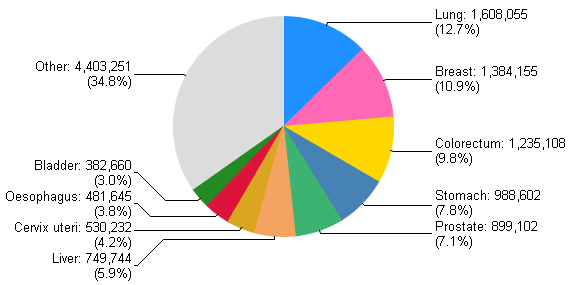
\includegraphics[width=.45\textwidth]{./images/statistics/repartitionCancerIncidence.png}}%
      \hfill%
      \subfigure[][\tiny \# of cancer deaths]{%
        \label{fig:stat1b}%
          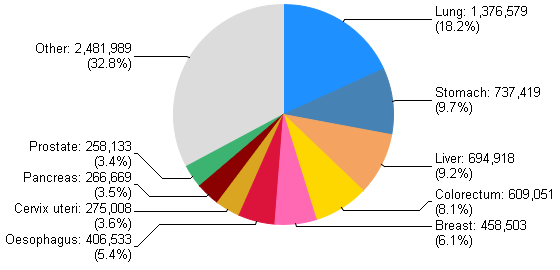
\includegraphics[width=.45\textwidth]{./images/statistics/repartitionCancerDeaths.png}}%
        \hspace*{\fill}%
      \label{fig:stat1}%
    \end{figure}
  \end{block}
  \begin{block}<2->{\small Implications}\footnotesize
    \begin{itemize}
    \item<2-> 2\textsuperscript{nd} most frequently diagnosed men cancer
    \item<3-> Accounting for $7.1\%$ of overall cancers diagnosed
    \item<3-> Accounting for $3.4\%$ of overall cancers death
    \end{itemize}
  \end{block}
\end{frame}

\subsection{Screening}

\begin{frame}
  \frametitle{Introduction}
  \framesubtitle{Screening}
  \begin{block}<1->{\small PSA level}\footnotesize
    $\rightarrow$ Checking for a higher-than-normal PSA level
    \begin{itemize}
    \item[\cross]<2-> Not reliable
    \end{itemize}
  \end{block}

  \begin{block}<3->{\small ``Blind'' TRUS biopsy}\footnotesize
    $\rightarrow$ Take several samples through biopsy at different prostate locations
    \begin{itemize}
    \item[\cross]<4-> Invasive procedure
    \item[\cross]<5-> Lead to false positives \& negatives
    \end{itemize}
  \end{block}

  \begin{block}<6->{\small Current trendy techniques: MRI}\footnotesize
    \begin{itemize}\small
    \item[\tick] Non-invasive technique
    \item[\cross] Need further investigations regarding the potential of the different MRI modalities available
    \end{itemize}
  \end{block}
\end{frame}

\subsection{MRI modalities}

\setcounter{subfigure}{0}% Reset subfigure counter

\begin{frame}
  \frametitle{Introduction}
  \framesubtitle{MRI modalities}
  \begin{block}{\small T$_2$W MRI}
    \begin{figure}%
      \centering
      \hspace*{\fill}%
      \subfigure[][\tiny Healthy]{%
        \label{fig:t2wh}%
        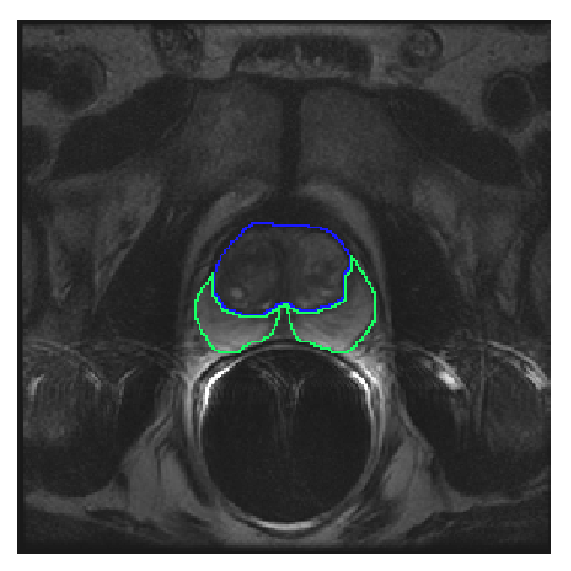
\includegraphics[width=.2\textwidth]{./images/mri/t2w/t2w_healthy.eps}}%
      \hfill%
      \subfigure[][\tiny CaP PZ]{%
        \label{fig:t2wcpz}%
        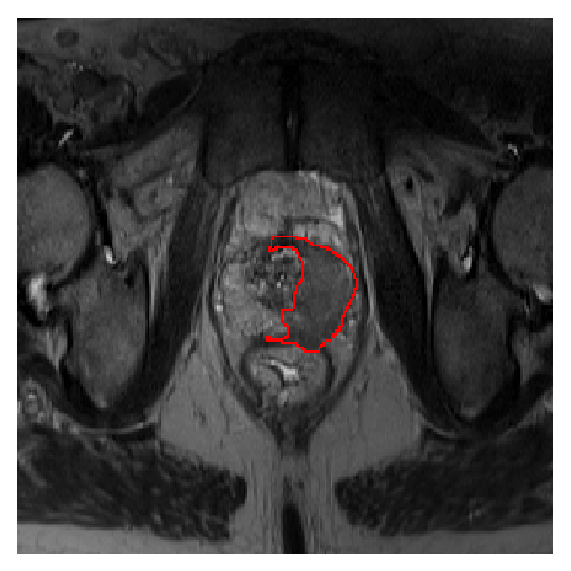
\includegraphics[width=.2\textwidth]{./images/mri/t2w/t2w_cancer_pz.eps}}%
      \hfill%
      \subfigure[][\tiny CaP CG]{%
        \label{fig:t2wccg}%
        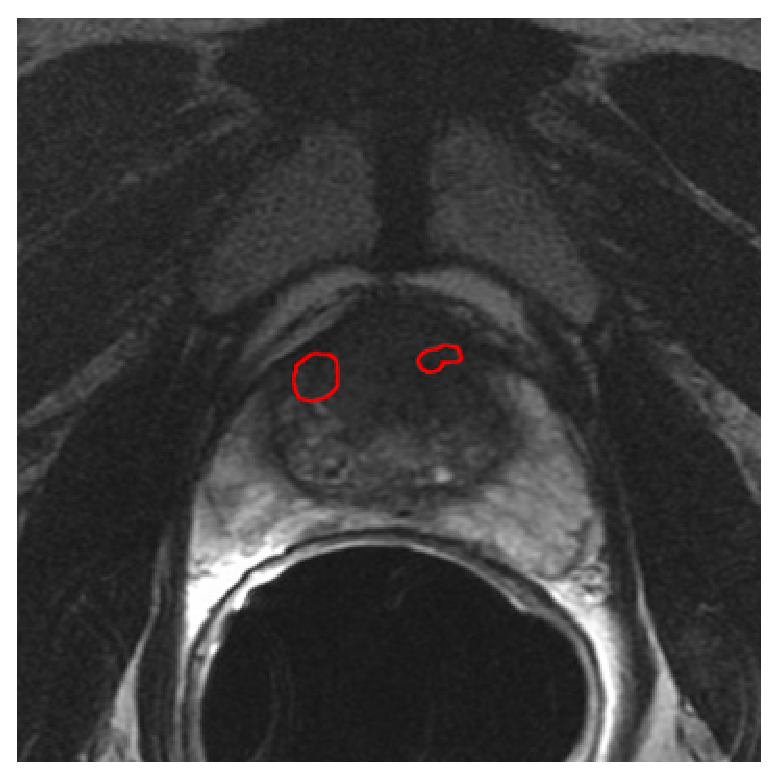
\includegraphics[width=.2\textwidth]{./images/mri/t2w/t2w_cancer_cg.eps}}%
      \hspace*{\fill}%
      \label{fig:t2w}%
    \end{figure}
  \end{block}
  \begin{redblock}{\small Features for CaP}\footnotesize
    \begin{itemize}
    \item Low-SI
    \item Ill-defined shape
    \end{itemize}
  \end{redblock}
\end{frame}

\setcounter{subfigure}{0}% Reset subfigure counter

\begin{frame}
  \frametitle{Introduction}
  \framesubtitle{MRI modalities}
  \begin{block}{\small DCE MRI}
    \begin{figure}%
      \centering
      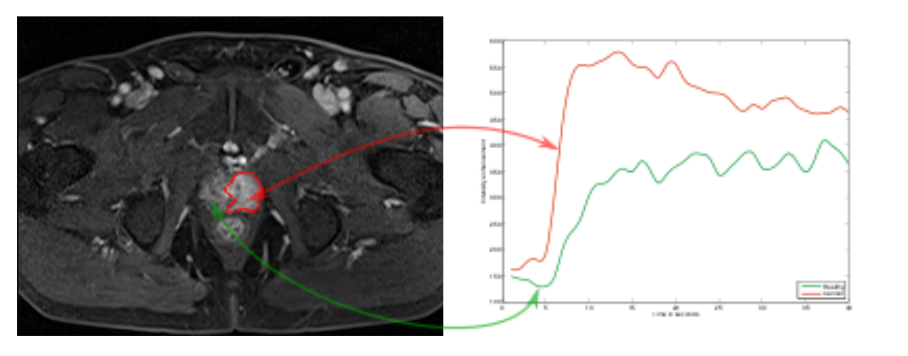
\includegraphics[width=.7\textwidth]{./images/mri/dce/dce_cancer_healthy_information.eps}
      \label{fig:dce}%
      \caption{{\color{green}Green}: healthy - {\color{red}Red}: CaP}
    \end{figure}
  \end{block}
  \begin{redblock}{\small Features for CaP}\footnotesize
    \begin{itemize}
    \item Faster wash-in, wash-out, time-to-peak enhancement
    \item Higher integral under the curve, max SI
    \end{itemize}
  \end{redblock}
\end{frame}

\setcounter{subfigure}{0}% Reset subfigure counter

\begin{frame}
  \frametitle{Introduction}
  \framesubtitle{MRI modalities}
  \begin{block}{\small DW MRI - ADC}
    \begin{figure}%
      \centering
      \hspace*{\fill}%
      \subfigure[][\tiny DW MRI]{%
        \label{fig:dw}%
        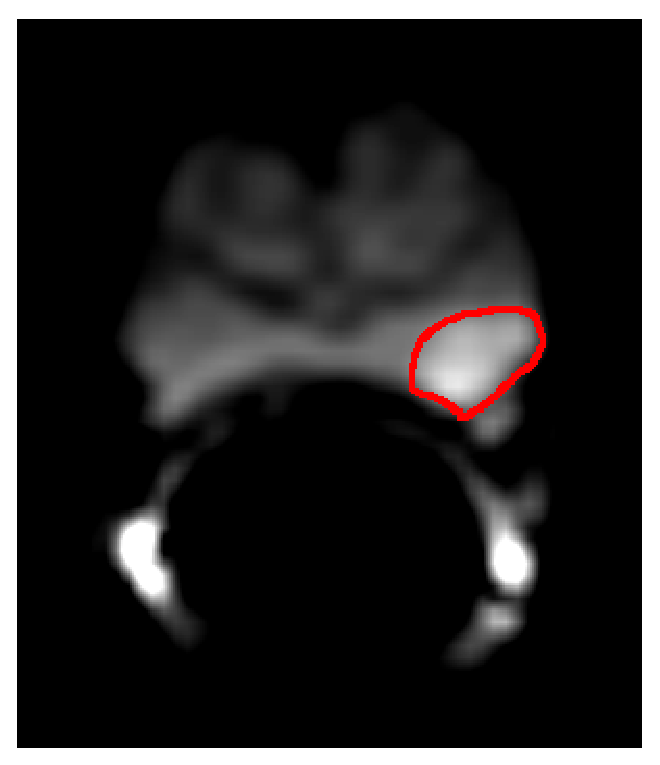
\includegraphics[width=.2\textwidth]{./images/mri/dwi/dwi_cancer.eps}}%
      \hfill%
      \subfigure[][\tiny ADC]{%
        \label{fig:adc}%
        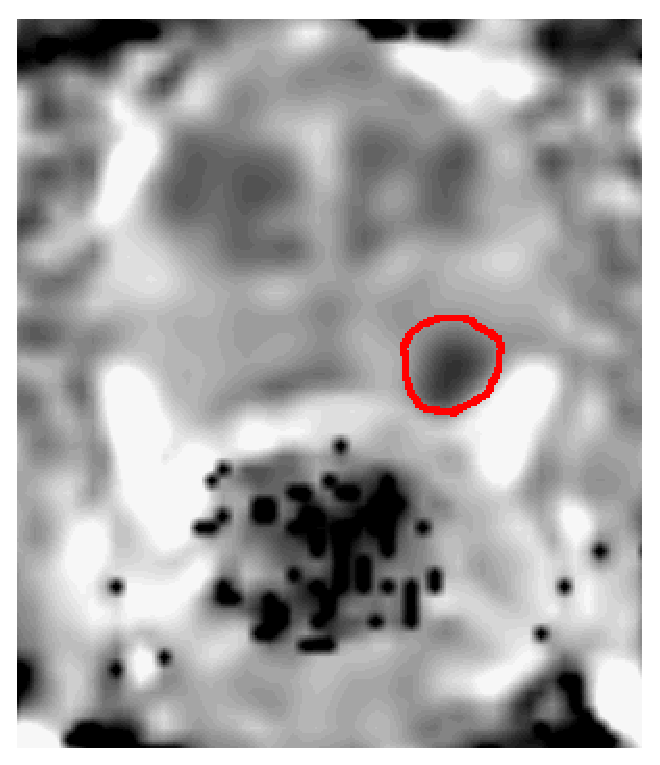
\includegraphics[width=.2\textwidth]{./images/mri/dwi/adc_cancer.eps}}%
      \hspace*{\fill}%
      \label{fig:dwadc}%
    \end{figure}
  \end{block}
  \begin{redblock}{\small Features for CaP}\footnotesize
    \begin{itemize}
    \item DW MRI - Higher SI
    \item ADC - Low-SI
    \end{itemize}
  \end{redblock}
\end{frame}

\setcounter{subfigure}{0}% Reset subfigure counter

\begin{frame}
  \frametitle{Introduction}
  \framesubtitle{MRI modalities}
  \begin{block}{\small MRSI}
    \begin{figure}%
      \centering
      \hspace*{\fill}%
      \subfigure[][\tiny Healthy]{%
        \label{fig:mrsih}%
        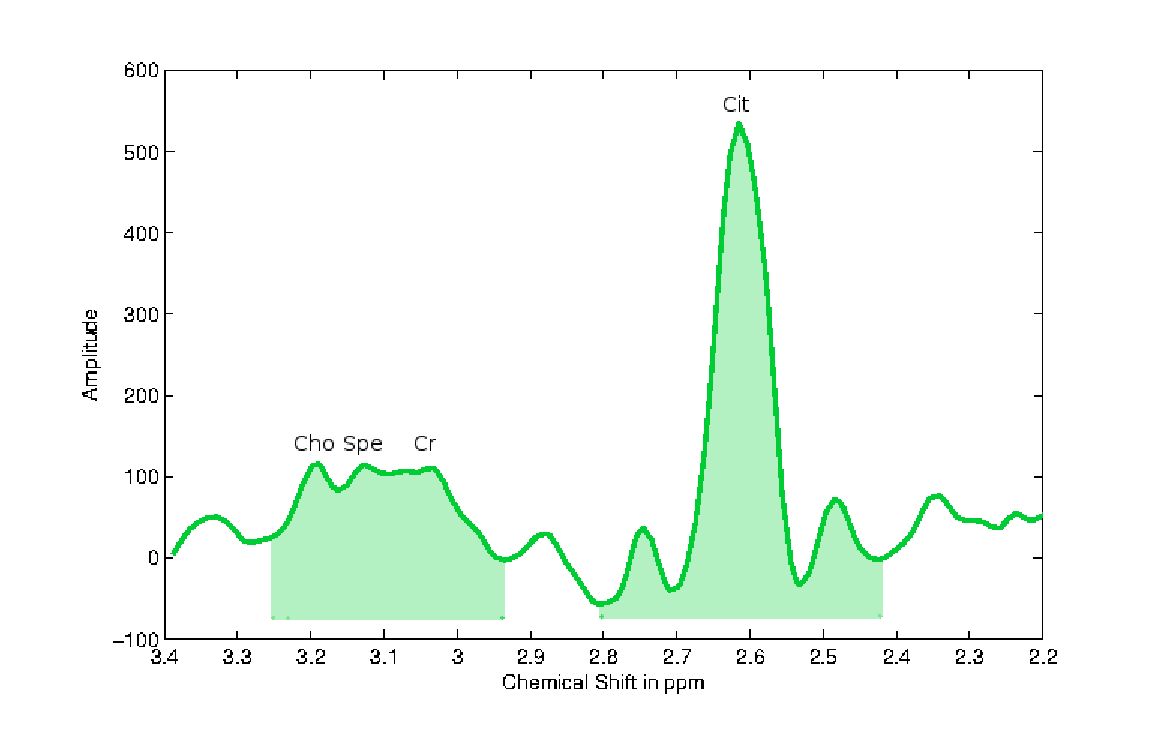
\includegraphics[width=.45\textwidth]{./images/mri/mrsi/mrsi_healthy.eps}}%
      \hfill%
      \subfigure[][\tiny CaP]{%
        \label{fig:mrsic}%
        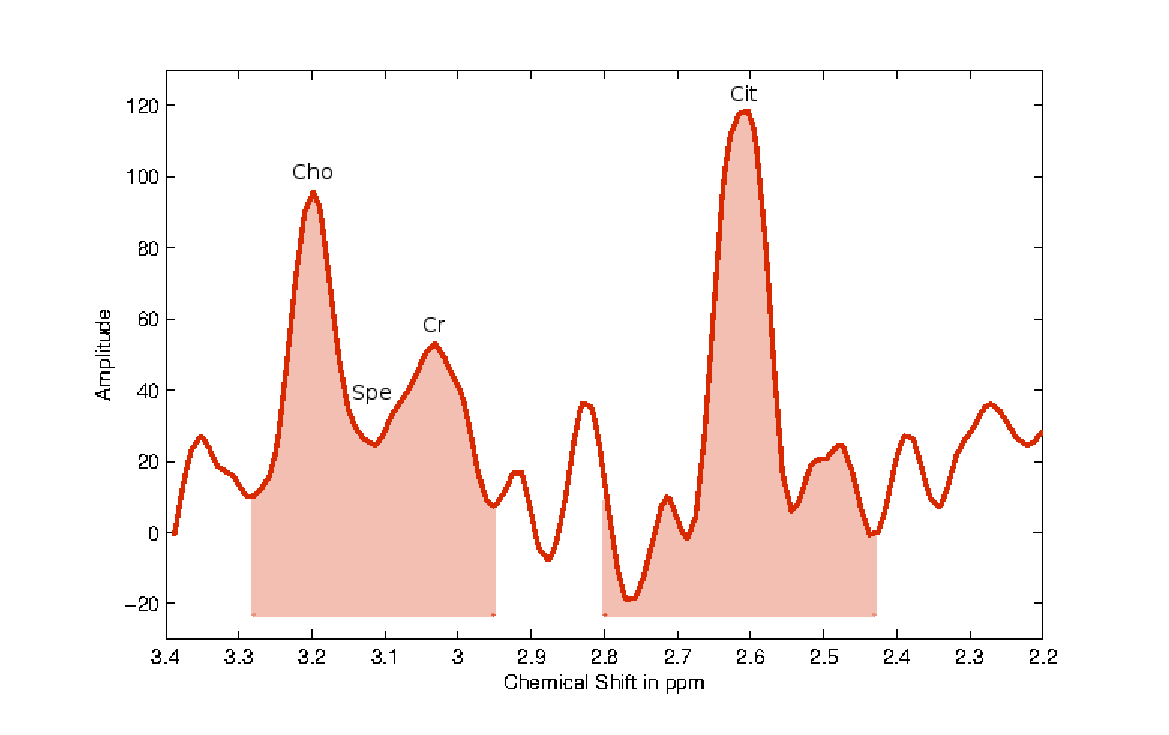
\includegraphics[width=.45\textwidth]{./images/mri/mrsi/mrsi_cancer.eps}}%
      \hspace*{\fill}%
      \label{fig:mrsi}%
    \end{figure}
  \end{block}
  \begin{redblock}{\small Features for CaP}\footnotesize
    \begin{itemize}
    \item Decrease of citrate and spermine
    \item Increase of choline
    \end{itemize}
  \end{redblock}
\end{frame}

\subsection{The MedIA evil}

\begin{frame}
  \frametitle{The Medical Imaging evil}
  \begin{block}<1->{\small The reasons of a nightmare}\footnotesize
    \begin{itemize}
    \item[$\rightarrow$] Multidisciplinary competences: medical doctors vs. computer scientists
    \end{itemize}
  \end{block}
  \begin{redblock}<2->{\small Some examples}\footnotesize
    \begin{itemize}
    \item Delay in the data acquisition
    \item Interest differences between the different core competences
    \item[$\rightarrow$] Lack of interest
    \end{itemize}
  \end{redblock}
  \begin{greenblock}<3->{\small The keystones needed}\footnotesize
    \begin{itemize}
    \item Common datasets
    \item Algorithms comparisons
    \item Full benchmarking
    \end{itemize}
  \end{greenblock}
\end{frame}

\section{I2CVB}

\subsection{Overview}

\begin{frame}
  \frametitle{Overview}
  \begin{block}{
\includegraphics[height=.04\textheight]{./images/i2cvb/i2cvb.pdf}\ Platform}
    \begin{figure}
      \centering
      
\includegraphics[width=.8\linewidth]{./images/i2cvb/website.pdf}
    \end{figure}
    \begin{itemize}
    \item Development of a web platform
    \end{itemize}
  \end{block}
\end{frame}

\begin{frame}
  \frametitle{Manifesto}
  \begin{columns}
    \column{.5\textwidth}
      \begin{block}{
\includegraphics[height=.04\textheight]{./images/i2cvb/i2cvb.pdf}\ Vision}
        \begin{figure}
          \centering
          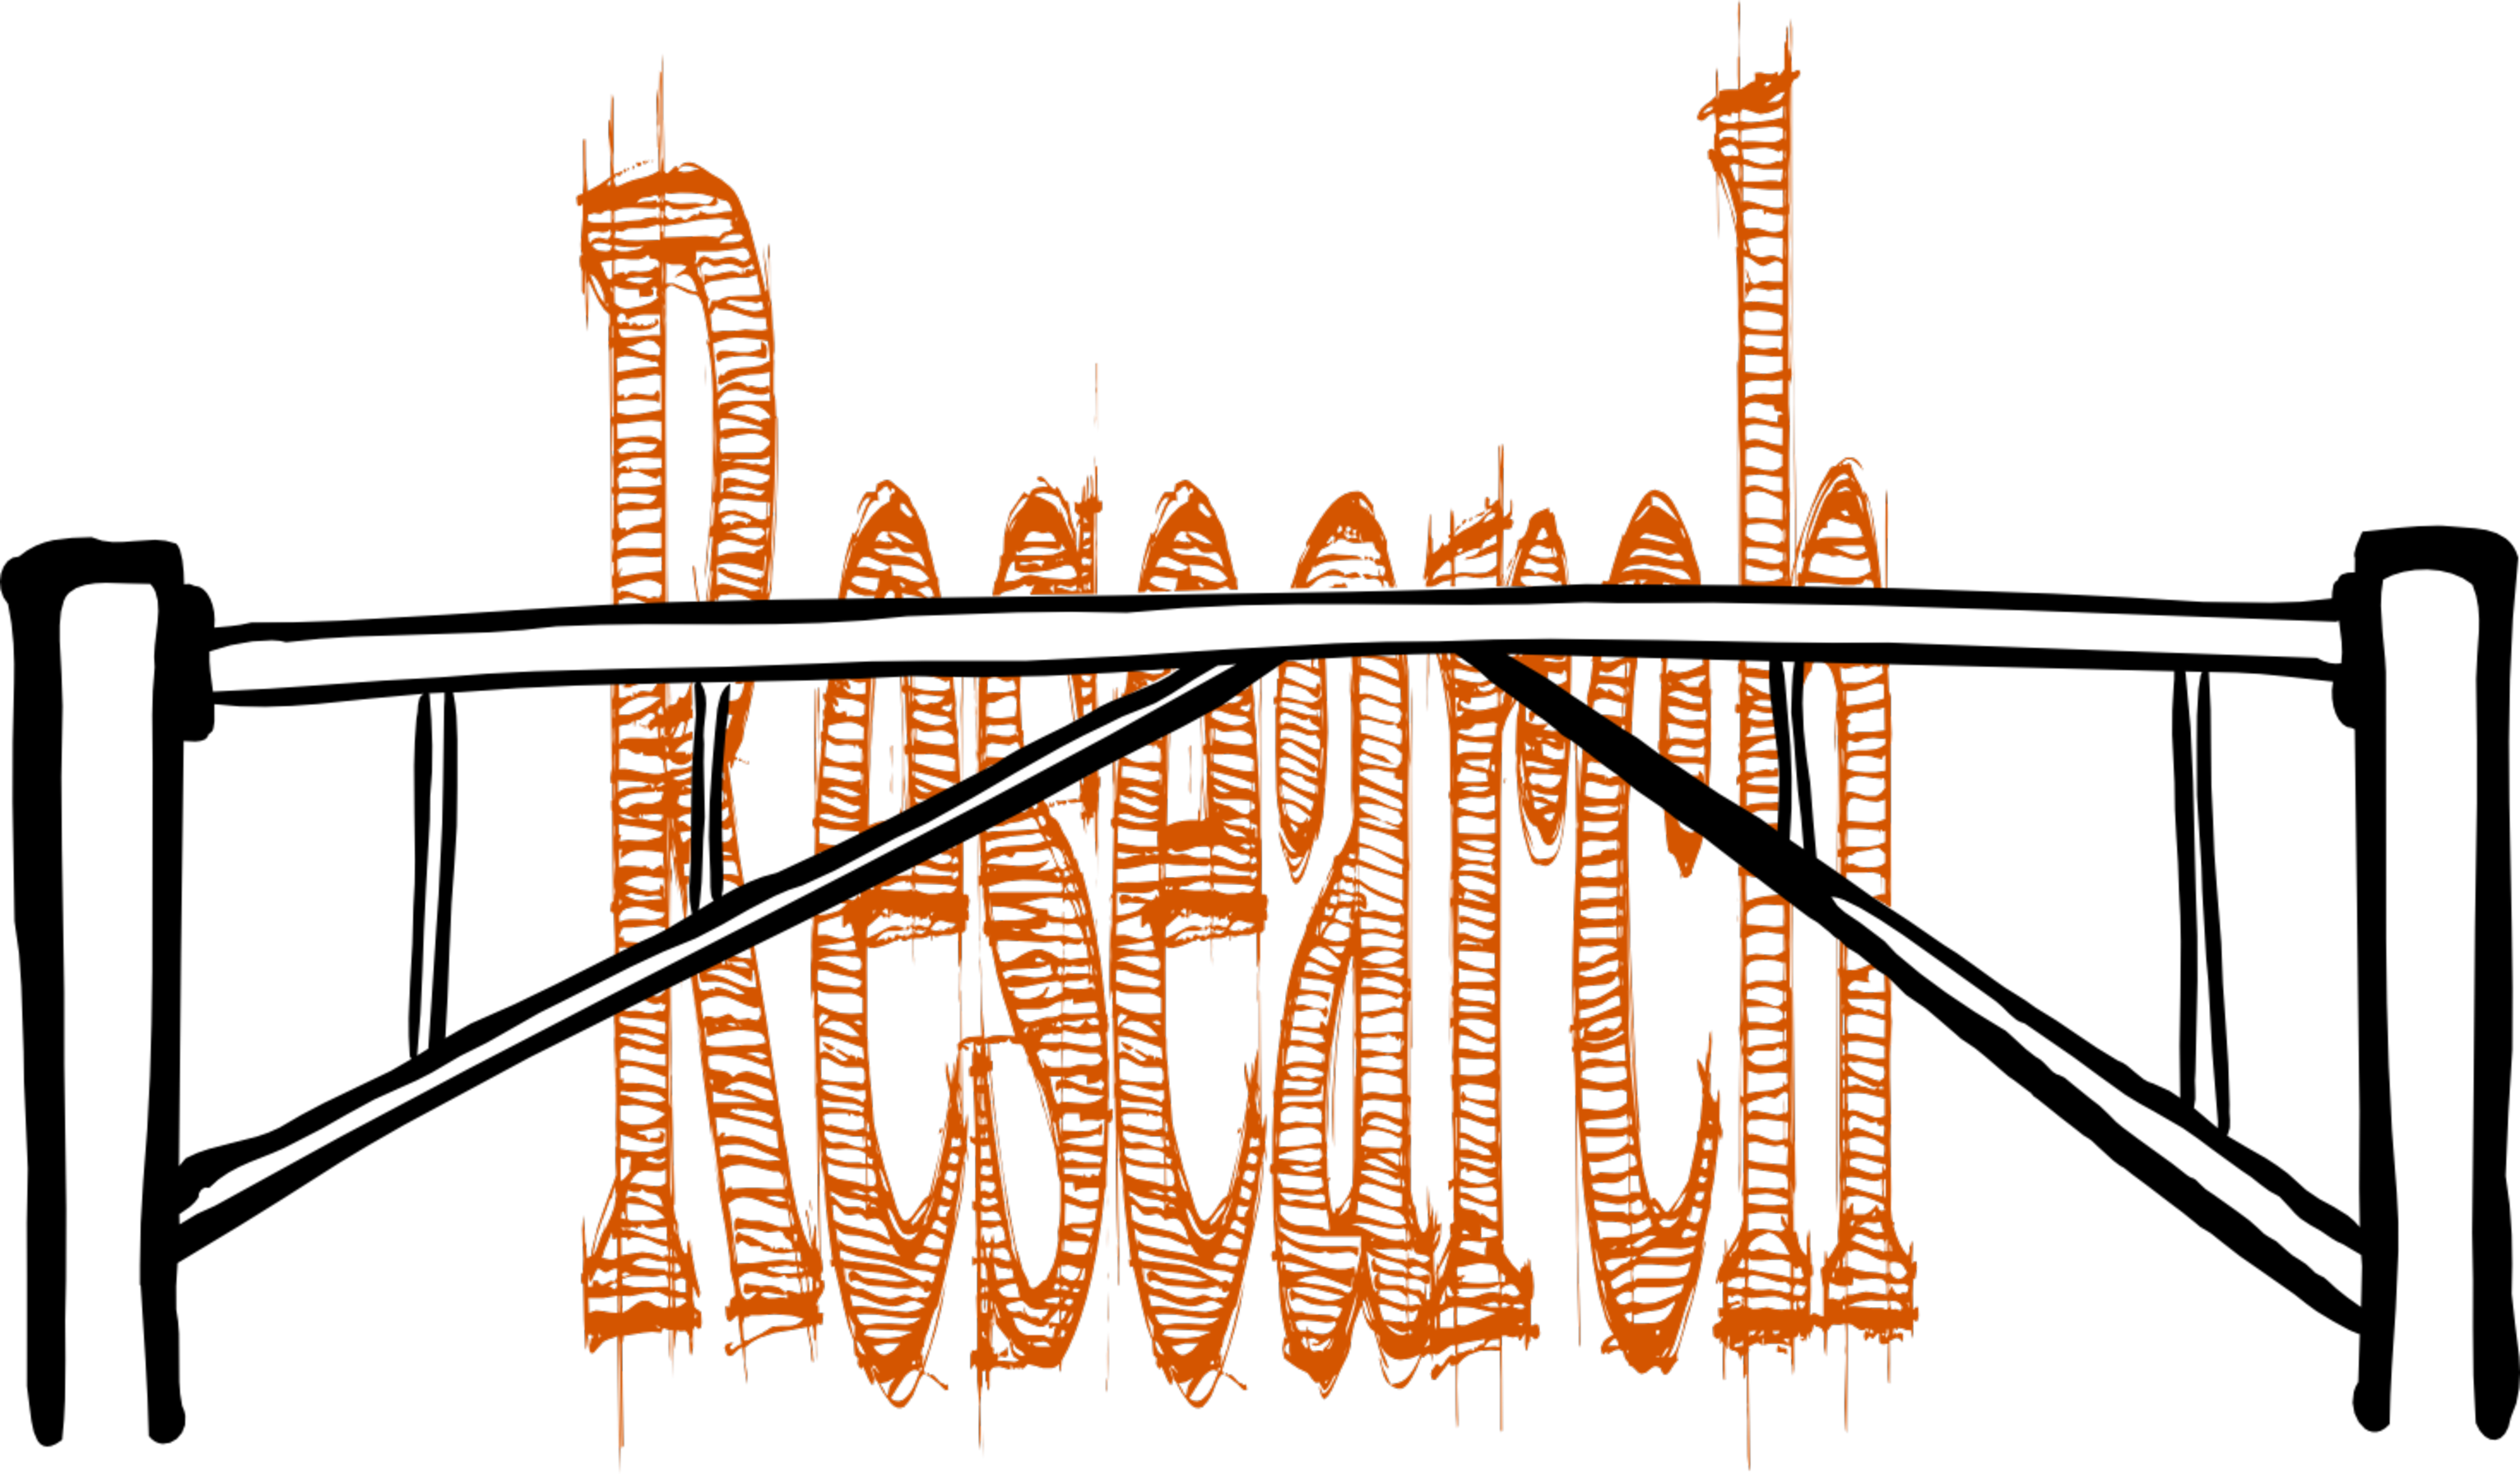
\includegraphics[height=.15\textheight]{./images/i2cvb/research.pdf}
        \end{figure}
        \vskip-4ex
        \begin{itemize}\tiny
        \item Democratization of the ability to research
        \end{itemize}
        \vskip1ex
      \end{block}
      \begin{block}{
\includegraphics[height=.04\textheight]{./images/i2cvb/i2cvb.pdf}\ Protagonists}
        \begin{figure}
          \centering
          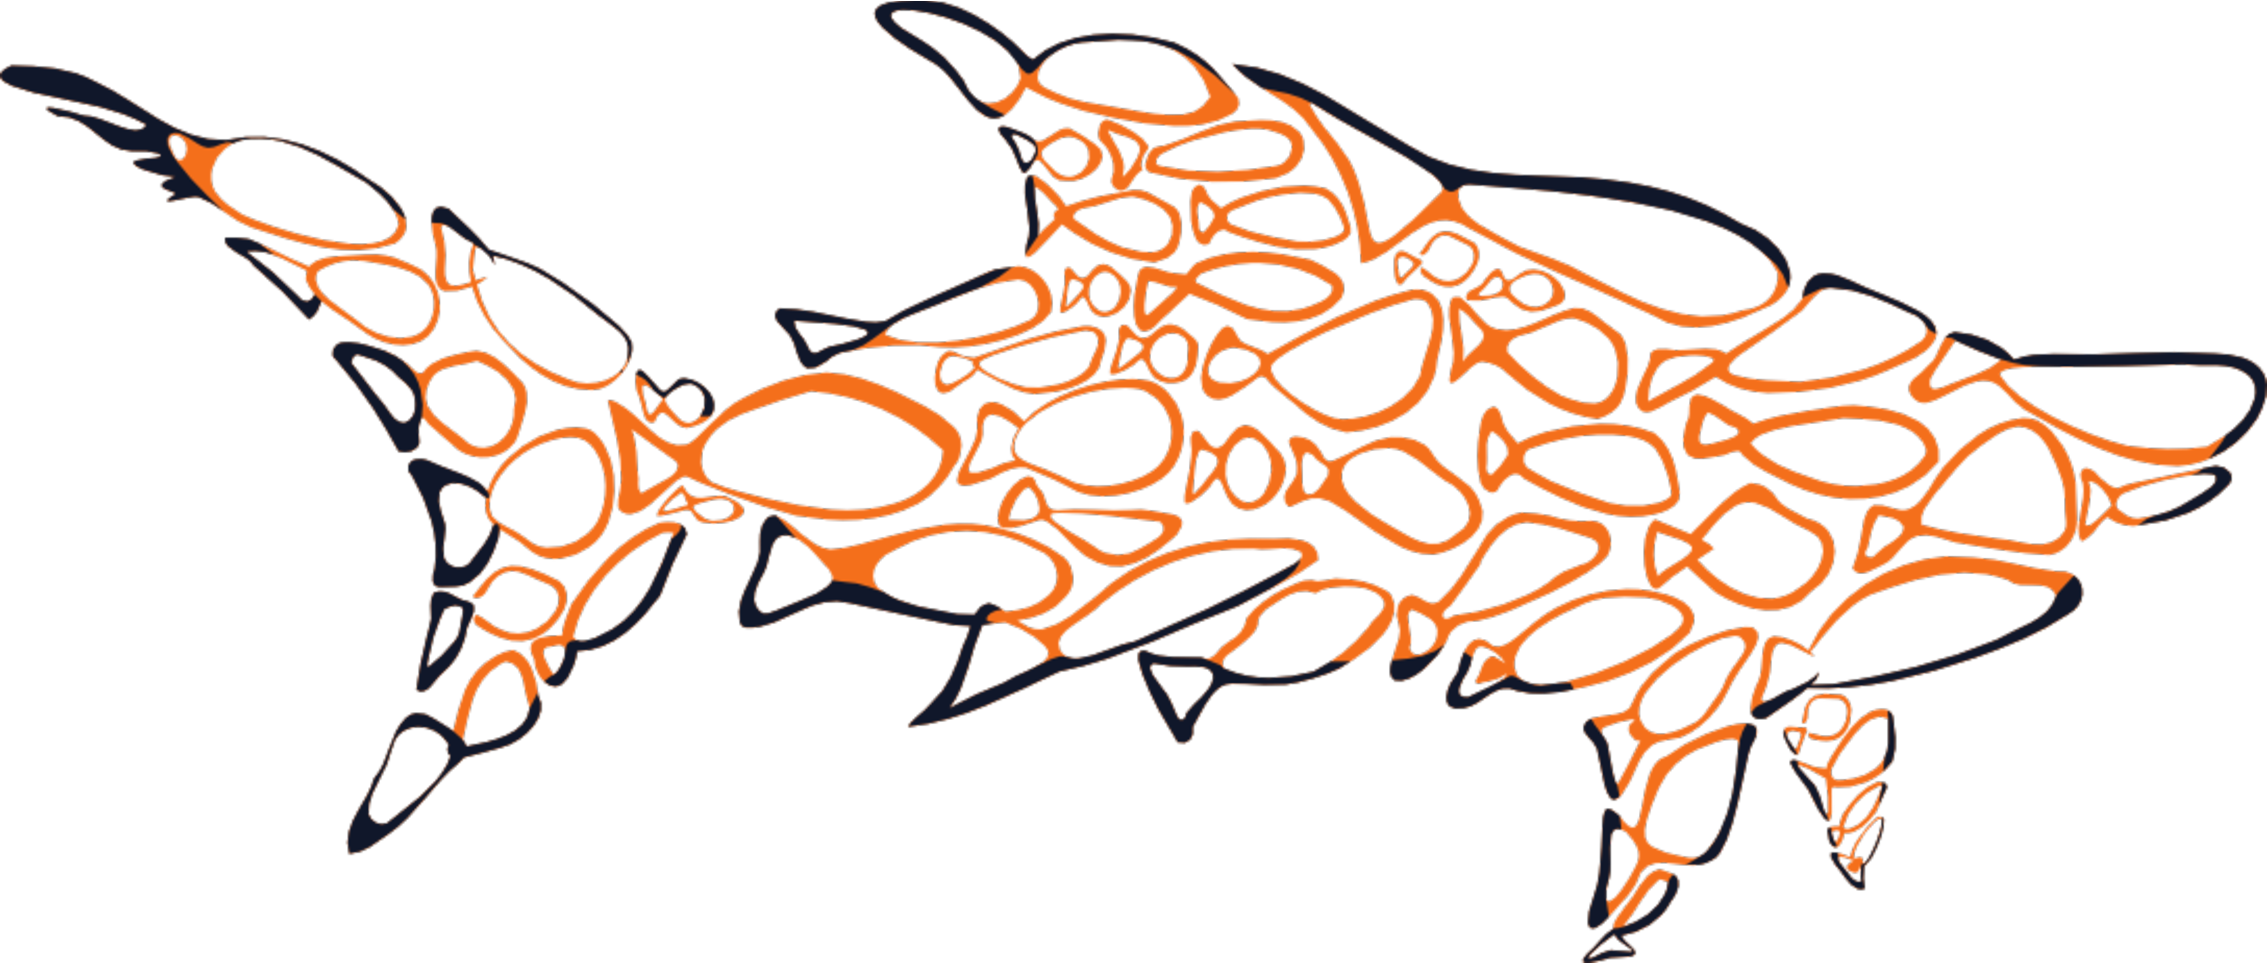
\includegraphics[height=.15\textheight]{./images/i2cvb/shark.pdf}
        \end{figure}
        \vskip-4ex
        \begin{itemize}\tiny
        \item Research groups and individuals from all walks of life to shape a transparent community
        \end{itemize}
      \end{block}
    \column{.5\textwidth}
      \begin{block}{
\includegraphics[height=.04\textheight]{./images/i2cvb/i2cvb.pdf}\ Mission}
        \begin{figure}
          \centering
          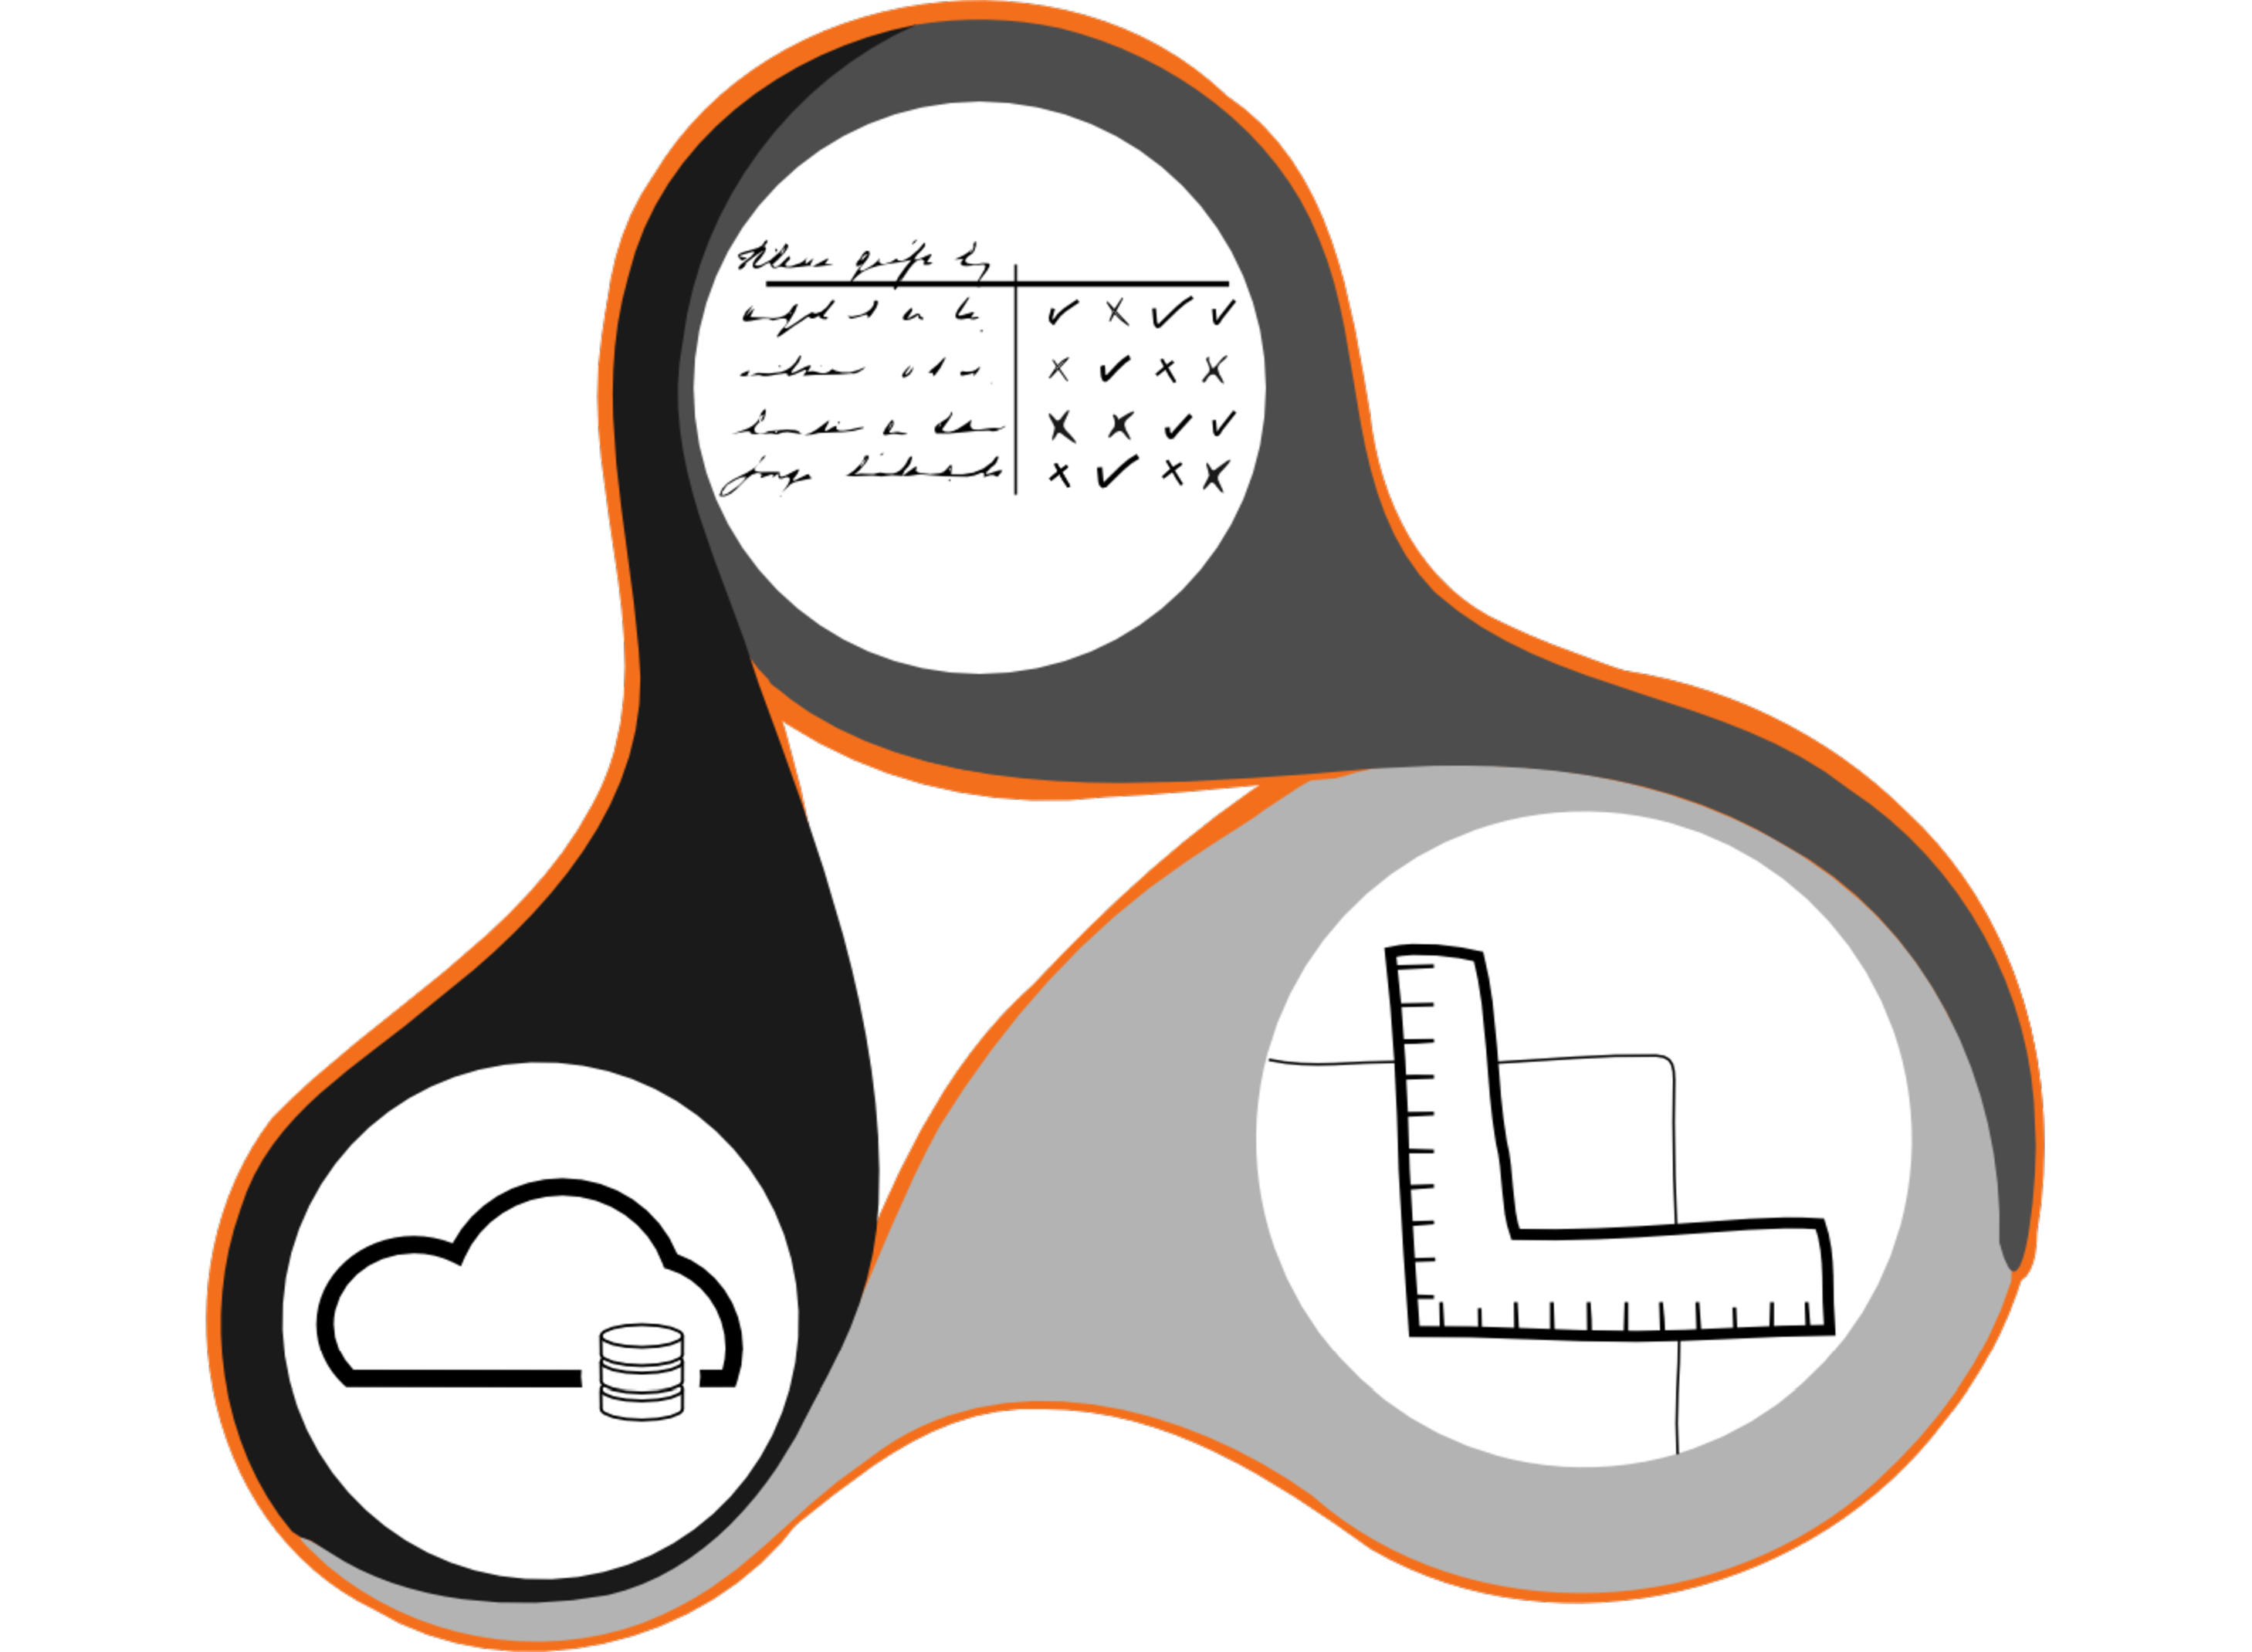
\includegraphics[height=.15\textheight]{./images/i2cvb/what.pdf}
        \end{figure}
        \vskip-4ex
        \begin{itemize}\tiny
        \item Open data; evaluation methods; comparison framework; reporting platform
        \end{itemize}
      \end{block}
      \begin{block}{
\includegraphics[height=.04\textheight]{./images/i2cvb/i2cvb.pdf}\ Strategy}
        \begin{figure}
          \centering
          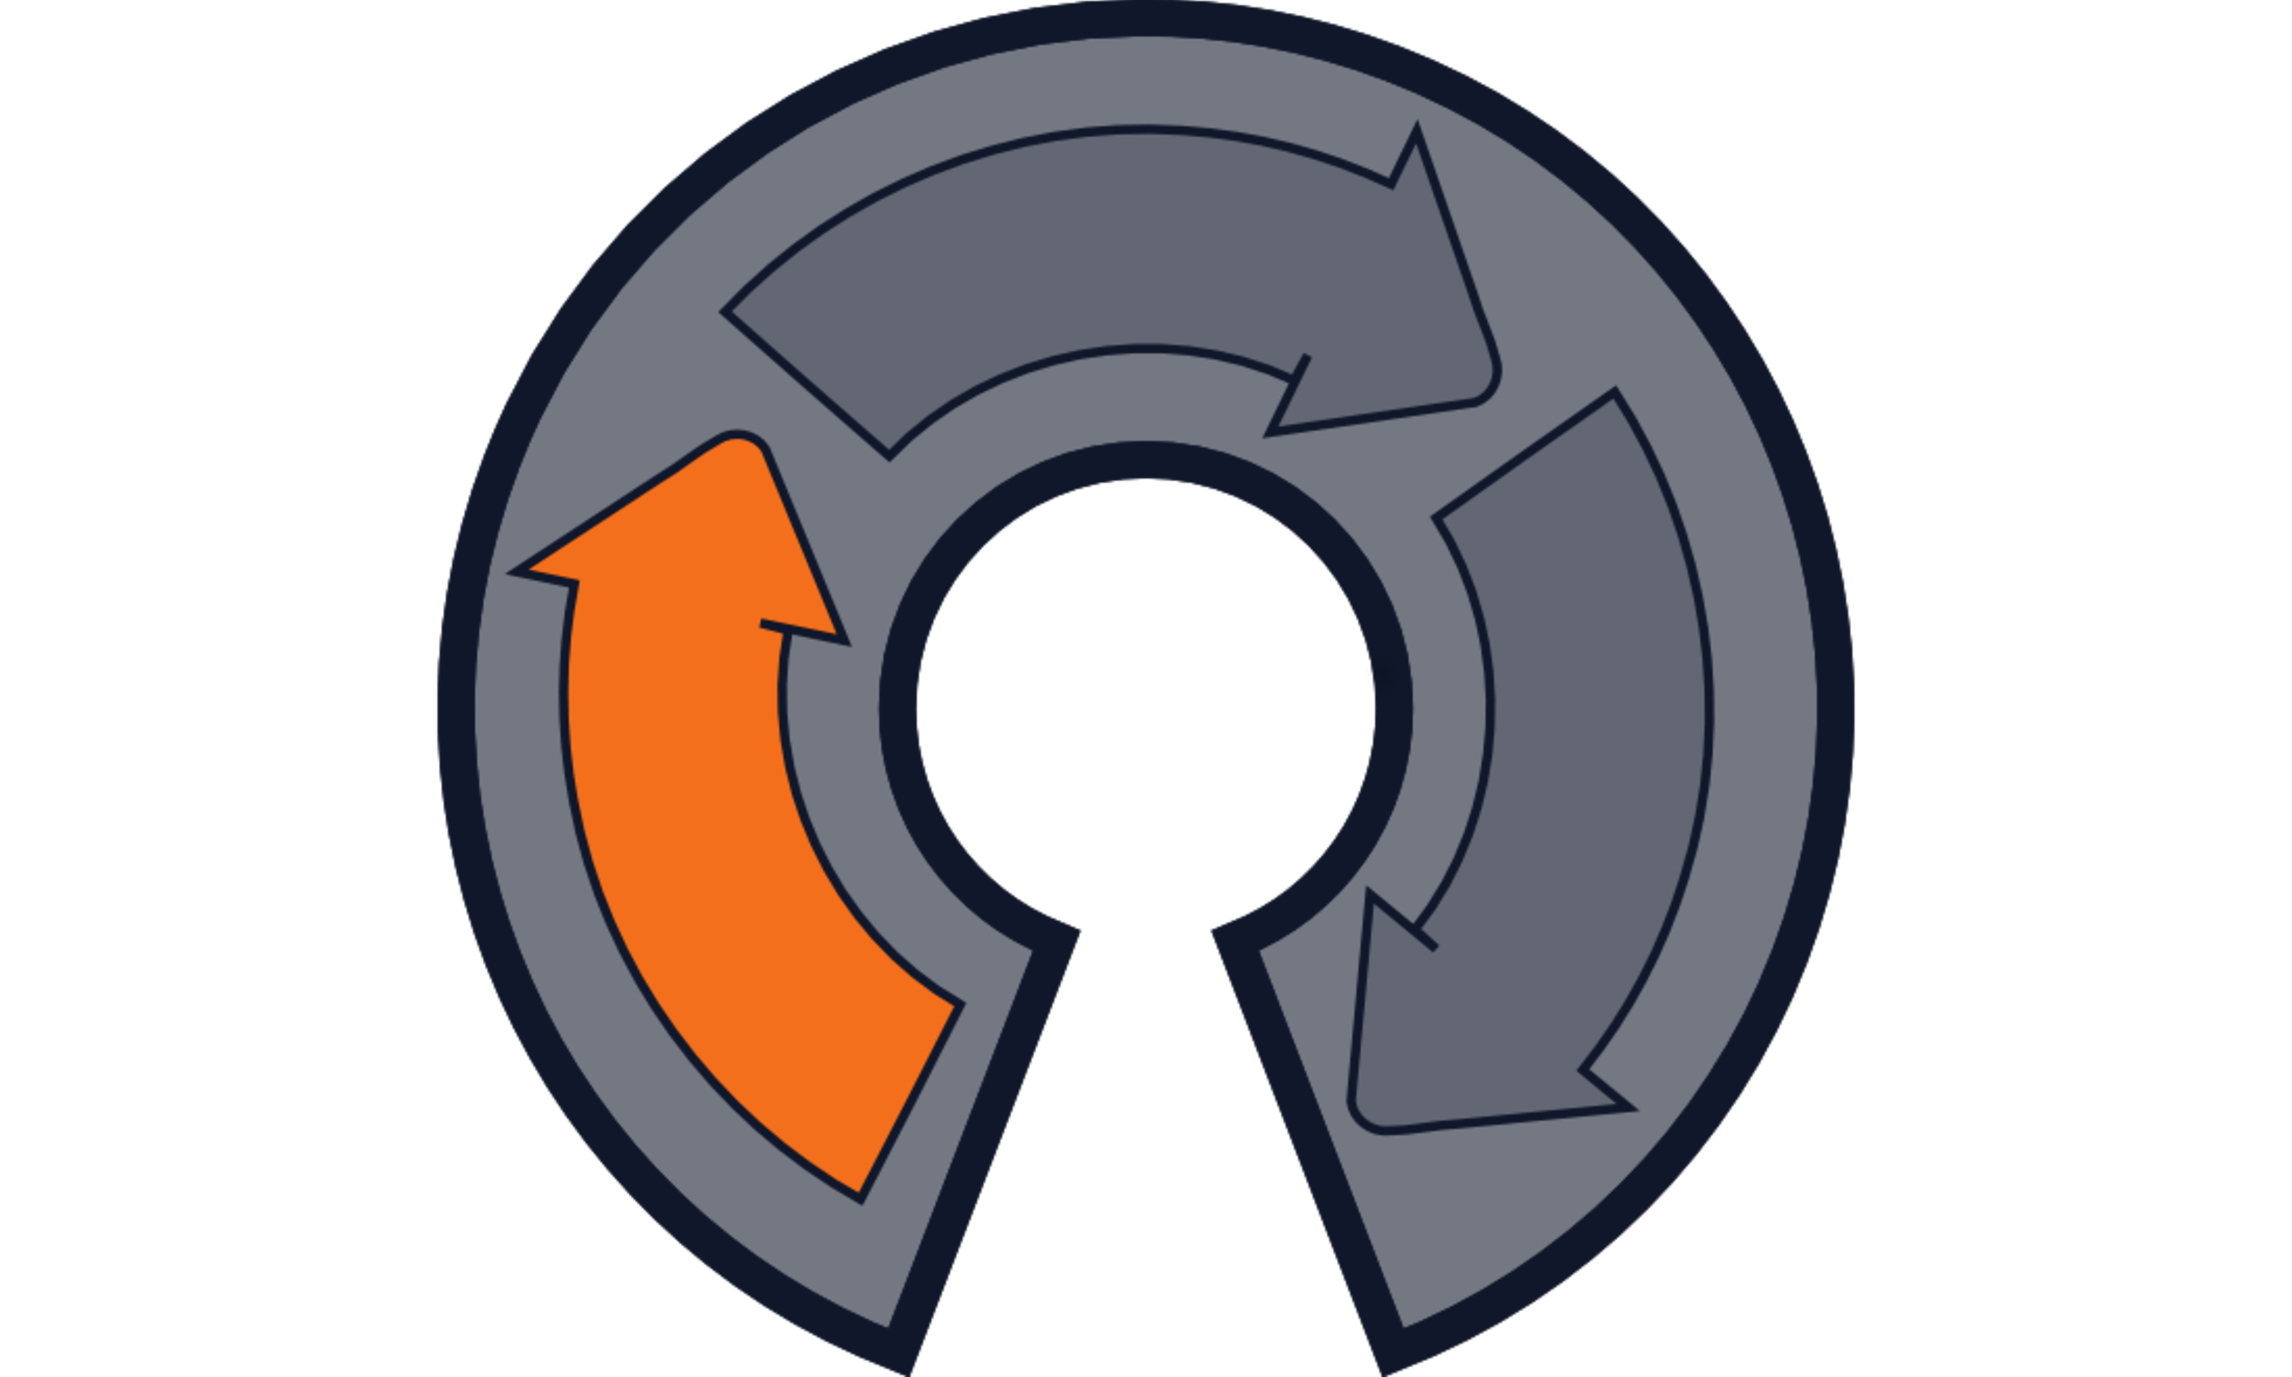
\includegraphics[height=.15\textheight]{./images/i2cvb/open.pdf}
        \end{figure}
        \vskip-4ex
        \begin{itemize}\tiny
        \item Transferring successful practises from Free Software and Quality Management
        \end{itemize}
        \vskip1ex
      \end{block}
  \end{columns}
\end{frame}

\subsection{Prostate dataset}

\begin{frame}
  \frametitle{I2CVB}
  \framesubtitle{Prostate dataset}
  \begin{block}{\small Multi-parametric MRI}\footnotesize
    \begin{itemize}
    \item Cohort of 20 patients
    \item T$_2$W MRI, DCE MRI \& ADC
    \item 3 Tesla whole body MRI without endorectal coil
    \end{itemize}
  \end{block}
  \begin{greenblock}{\small Ground-truth}\footnotesize
    \begin{itemize}
    \item Delineations: prostate - zones - CaP
    \item Healthy: 2 \textit{vs.} CaP: \{PZ: 13, CG: 3, PZ + CG: 2 \}
    \end{itemize}
  \end{greenblock}
\end{frame}

\section{Classification framework}

\begin{frame}
  \frametitle{Classification framework}
  \begin{block}{\small Pre-processing}\footnotesize
    \begin{itemize}
    \item Resampling data to T$_2$W MRI dataset
    \item Balancing data using random sampling without replacement
    \item[$\rightarrow$] 218,423 voxels
    \end{itemize}
  \end{block}
  \begin{block}{\small Features extraction}\footnotesize
    \begin{itemize}
    \item Voxel-based ``$V(\cdot)$'': intensities of T$_2$W~MRI, ADC, DCE~MRI \& zonal information (PZ \textit{vs.} CG)
    \item 3D-texton-based ``$T(\cdot)$'': ($9 \times 9 \times 3$) intensities of T$_2$W~MRI, ADC, DCE~MRI \& zonal information (PZ \textit{vs.} CG)
    \end{itemize}
  \end{block}
  \begin{block}{\small Features classification}\footnotesize
    \begin{itemize}
    \item[$\rightarrow$] Gradient Boosted Trees classifier
    \end{itemize}
  \end{block}
\end{frame}

\section{Results}

\subsection{Sensitivity \& specificity}

\setcounter{subfigure}{0}% Reset subfigure counter

\begin{frame}
  \frametitle{Results}
  \begin{block}{\small Sensitivity \& Specificity}\footnotesize
    %% Figure 1
\begin{figure}[t]
%%Figure1a
\subfigure[][\tiny Voxel-based]{\label{fig:voxres}
\hspace{0.8cm}
\begin{tikzpicture} [scale=.45,every node/.style={scale=0.45}]  %[scale=.68]

\def\labels{
{\color{green}$V_{1}$}, 
{\color{green}$V_{2}$}, 
{\color{green}$V_{3}$},  
{\color{green}$V_{4}$},
{\color{green}$V_{5}$},
{\color{green}$V_{6}$},
{\color{green}$V_{7}$},
{\color{green}$V_{8}$}
 }

\def\reward{85.1,77.6,76.0,78.8,75.8,80.4,82.6,84.3}
\def\spec{46.7,60.7,76.8,63.4,76.8,77.8,78.2,81.7}
\def\cZoom{2.5} 
\def\percentageLabelAngle{10}
\def\nbeams{8}
\pgfmathsetmacro\beamAngle{(360/\nbeams)}
\pgfmathsetmacro\halfAngle{(180/\nbeams)}

\pgfmathsetmacro\globalRotation{\halfAngle}

\foreach \n  [count=\ni] in \labels
{
\pgfmathsetmacro\cAngle{{(\ni*(360/\nbeams))+\globalRotation}}
\draw(\cAngle:{\cZoom*1.00})  node[fill=white] {\n};
\draw [thin] (0,0) -- (\cAngle:{\cZoom*0.9}) ;

}

%% draw the % rings 
\foreach \x in {12.5,25, ...,100} 
\draw [thin,color=gray!50] (0,0) circle [radius={\cZoom*\x/110}];

\foreach \x in {50,75,100}
{ 
     \draw [thin,color=black!50] (0,0) circle [radius={\cZoom/110*\x}];
     \foreach \a in {0, 180} \draw ({\percentageLabelAngle+\a}:{\cZoom*0.01*\x}) node  [inner sep=0pt,outer sep=0pt,fill=white,font=\fontsize{3}{3.5}\selectfont]{$\x\%$};
}

%% draw the path of the percentages
\def\aux{{\reward}}
\pgfmathsetmacro\origin{\aux[\nbeams-1]} 
\draw [blue, thick] (\globalRotation:{\cZoom*\origin/110}) \foreach \n  [count=\ni] in \reward { -- ({(\ni*(360/\nbeams))+\globalRotation}:{\cZoom*\n/110}) } ;

\def\auxx{{\spec}}
\pgfmathsetmacro\origin{\auxx[\nbeams-1]} 
\draw [red, thick] (\globalRotation:{\cZoom*\origin/110}) \foreach \n  [count=\ni] in \spec { -- ({(\ni*(360/\nbeams))+\globalRotation}:{\cZoom*\n/110}) };


\foreach \n [count=\ni] in \reward 
{
  \pgfmathsetmacro\cAngle{{(\ni*(360/\nbeams))+\globalRotation}}
  \pgfmathsetmacro\nreward{\aux[\ni-1]}
  \pgfmathsetmacro\nspec{\auxx[\ni-1]}
  \draw (\cAngle:{\cZoom*1.36}) node[align=center] {{\color{blue}\nreward $\%$ } \\{ \color{red}\nspec $\%$}};
};

%%%% draw the domain of each class 
\def\puta{3/0/{Mono-parametric},
  5/3/{Multi-parametric}}
\foreach \numElm/\contadorQueNoSeCalcular/\name [count=\ni] in \puta
 {

   \pgfmathsetmacro\initialAngle{(\contadorQueNoSeCalcular*\beamAngle)+\halfAngle+\globalRotation}
   \pgfmathsetmacro\finalAngle  {((\numElm+\contadorQueNoSeCalcular)*\beamAngle)+\halfAngle+\globalRotation}
   \pgfmathsetmacro\l  {\cZoom*1.5+.3pt}
   \draw (\initialAngle:{\cZoom*1.6}) -- (\initialAngle:{\cZoom*1.1});
   \draw [ |<->|,>=latex] (\initialAngle:\l) arc (\initialAngle:\finalAngle:\l) ;     
   \pgfmathsetmacro\r  {\cZoom*1.5+.45pt}
   {\draw [decoration={text along path,  text={\name},text align={center}},decorate] (\finalAngle:\r) arc (\finalAngle:\initialAngle:\r);} 
    
  }  
\end{tikzpicture} 
}\hfill
%%Figure1b
\subfigure[][\tiny 3D-texton-based]{\label{fig;texres}
\begin{tikzpicture} [scale=.45,every node/.style={scale=0.45}]  %[scale=.68]

\def\labels{
{\color{green}$T_{1}$}, 
{\color{green}$T_{2}$}, 
{\color{green}$T_{3}$},  
{\color{green}$T_{4}$},
{\color{green}$T_{5}$},
{\color{green}$T_{6}$},
{\color{green}$T_{7}$},
{\color{green}$T_{8}$}
 }

\def\reward{82.5,83.2,91.1,87.5,93.4,93.4,94.2,94.7}
\def\spec{76.7,73.5,89.2,83.3,90.7,90.9,91.6,93.0}
\def\cZoom{2.5} 
\def\percentageLabelAngle{10}
\def\nbeams{8}
\pgfmathsetmacro\beamAngle{(360/\nbeams)}
\pgfmathsetmacro\halfAngle{(180/\nbeams)}

\pgfmathsetmacro\globalRotation{\halfAngle}

\foreach \n  [count=\ni] in \labels
{
\pgfmathsetmacro\cAngle{{(\ni*(360/\nbeams))+\globalRotation}}
\draw(\cAngle:{\cZoom*1.00})  node[fill=white] {\n};
\draw [thin] (0,0) -- (\cAngle:{\cZoom*0.9}) ;

}

% draw the % rings 
\foreach \x in {12.5,25, ...,100} 
\draw [thin,color=gray!50] (0,0) circle [radius={\cZoom*\x/110}];

\foreach \x in {50,75,100}
{ 
     \draw [thin,color=black!50] (0,0) circle [radius={\cZoom/110*\x}];
     \foreach \a in {0, 180} \draw ({\percentageLabelAngle+\a}:{\cZoom*0.01*\x}) node  [inner sep=0pt,outer sep=0pt,fill=white,font=\fontsize{3}{3.5}\selectfont]{$\x\%$};
}


% draw the path of the percentages
\def\aux{{\reward}}
\pgfmathsetmacro\origin{\aux[\nbeams-1]} 
\draw [blue, thick] (\globalRotation:{\cZoom*\origin/110}) \foreach \n  [count=\ni] in \reward { -- ({(\ni*(360/\nbeams))+\globalRotation}:{\cZoom*\n/110}) } ;


\def\auxx{{\spec}}
\pgfmathsetmacro\origin{\auxx[\nbeams-1]} 
\draw [red, thick] (\globalRotation:{\cZoom*\origin/110}) \foreach \n  [count=\ni] in \spec { -- ({(\ni*(360/\nbeams))+\globalRotation}:{\cZoom*\n/110}) };

% label all the percentags
\foreach \n [count=\ni] in \reward 
{
  \pgfmathsetmacro\cAngle{{(\ni*(360/\nbeams))+\globalRotation}}
  \pgfmathsetmacro\nreward{\aux[\ni-1]}
  \pgfmathsetmacro\nspec{\auxx[\ni-1]}
  \draw (\cAngle:{\cZoom*1.36}) node[align=center] {{\color{blue}\nreward $\%$ } \\{ \color{red}\nspec $\%$}};
};

%%% draw the domain of each class 
\def\puta{3/0/{Mono-parametric},
  5/3/{Multi-parametric}}
\foreach \numElm/\contadorQueNoSeCalcular/\name [count=\ni] in \puta
 {
   \pgfmathsetmacro\initialAngle{(\contadorQueNoSeCalcular*\beamAngle)+\halfAngle+\globalRotation}
   \pgfmathsetmacro\finalAngle  {((\numElm+\contadorQueNoSeCalcular)*\beamAngle)+\halfAngle+\globalRotation}
   \pgfmathsetmacro\l  {\cZoom*1.5+.3pt}
   \draw (\initialAngle:{\cZoom*1.6}) -- (\initialAngle:{\cZoom*1.1});
   \draw [ |<->|,>=latex] (\initialAngle:\l) arc (\initialAngle:\finalAngle:\l) ;     
   \pgfmathsetmacro\r  {\cZoom*1.5+.45pt}
   {\draw [decoration={text along path,  text={\name},text align={center}},decorate] (\finalAngle:\r) arc (\finalAngle:\initialAngle:\r);}     
  }  
\end{tikzpicture}
}
\label{fig:result}
\end{figure}

%%% Local Variables: 
%%% mode: latex
%%% TeX-master: "../../master.tex"
%%% End: 
  \end{block}
\end{frame}

\subsection{ROC curves}

\setcounter{subfigure}{0}% Reset subfigure counter

\begin{frame}
  \frametitle{Results}
  \begin{block}{\small ROC curves}\footnotesize
        \begin{figure}%
      \centering
      \hspace*{\fill}%
      \subfigure[][\tiny Voxel-based]{%
        \label{fig:rocv}%
        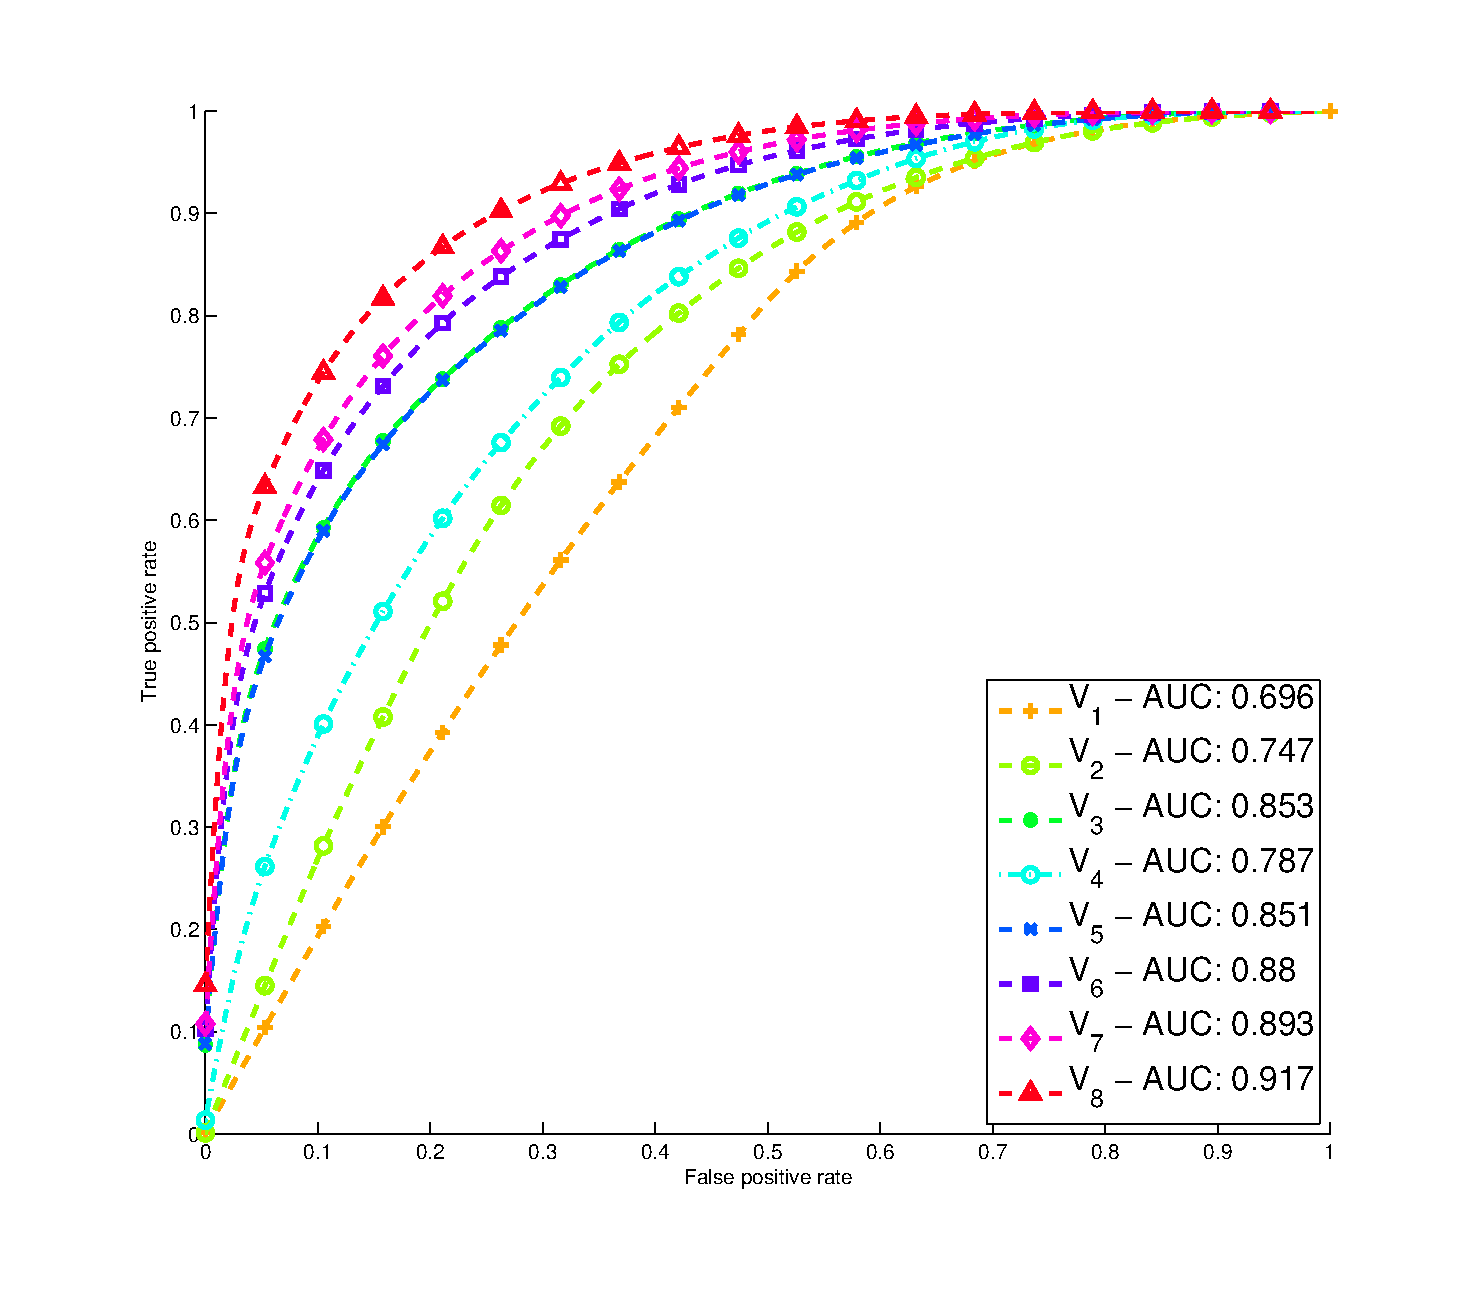
\includegraphics[width=.45\textwidth]{./images/results/voxel-roc.eps}}%
      \hfill%
      \subfigure[][\tiny 3D-texton-based]{%
        \label{fig:roct}%
        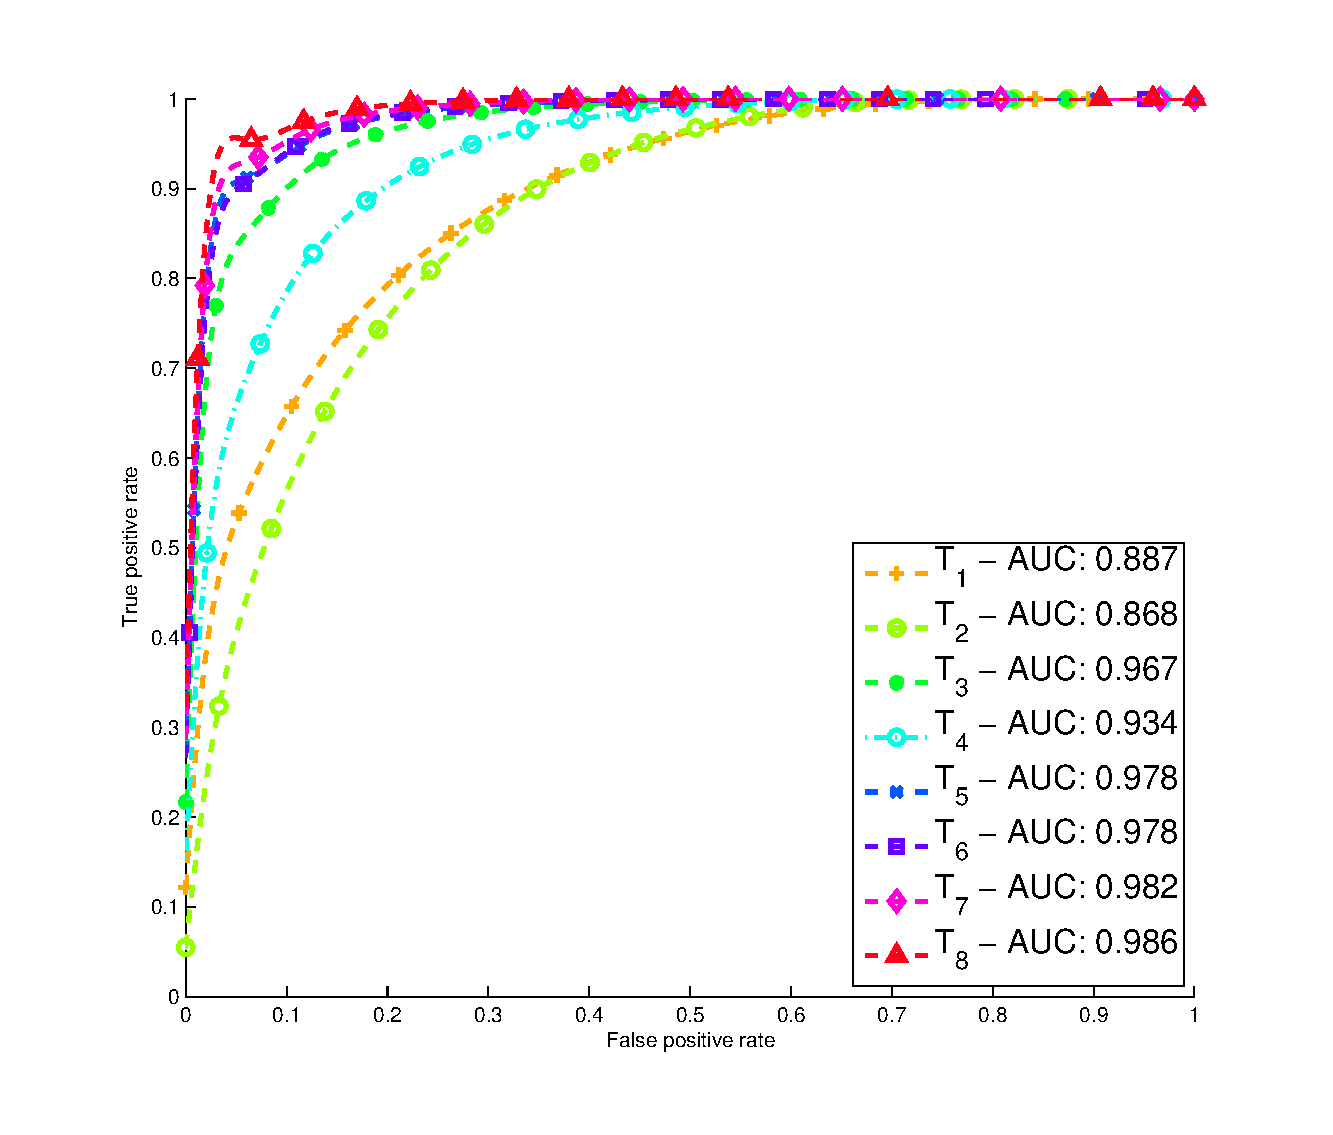
\includegraphics[width=.45\textwidth]{./images/results/texton-roc.eps}}%
      \hspace*{\fill}%
      \label{fig:roc}%
    \end{figure}
  \end{block}
\end{frame}

\section{Conclusion}

\begin{frame}
  \frametitle{Conclusion}
  \begin{greenblock}{\small Discussions}\footnotesize
    \begin{itemize}
    \item DCE~MRI is the most disciminative feature
    \item Combinations of all the modalities lead to better performance
    \item 3D-texton and neighbourhood information significantly improve the performace
    \end{itemize}
  \end{greenblock}
  \begin{redblock}{\small Future works}\footnotesize
    \begin{itemize}
    \item Normalisation of the data in a patient-based fashion
    \item Use more complex features
    \item Perform LOPO cross-validation
    \item Perform a full benchmark study of the current methods!!!!
    \end{itemize}
  \end{redblock}
\end{frame}

\section*{References}

\begin{frame}[allowframebreaks]
        \frametitle{References}
        \nocite{Ferlay2010,Siegel2014,Etzioni2002,Chou2011,Andriole2009,Hugosson2010,Schroeder2012,Lemaitre2015,Litjens2011,Litjens2012a,Litjens2014,Liu2013,Peng2013,Viswanath2011,johnson2013,Becker2013,Friedman1999,Friedman2000,Freund1997,Zheng2008,Chan2003,Zhang2005,Caruana2006}
        \bibliographystyle{apalike}
        \bibliography{literature_review.bib}
\end{frame}


\end{document}